\chapter{仿真}
\label{cha:intro}
在Multisim中,依据电路原理图搭建电路进行仿真测试
\section{红外发射Multisim仿真电路}
\begin{figure}[H] % use float package if you want it here
    \centering
    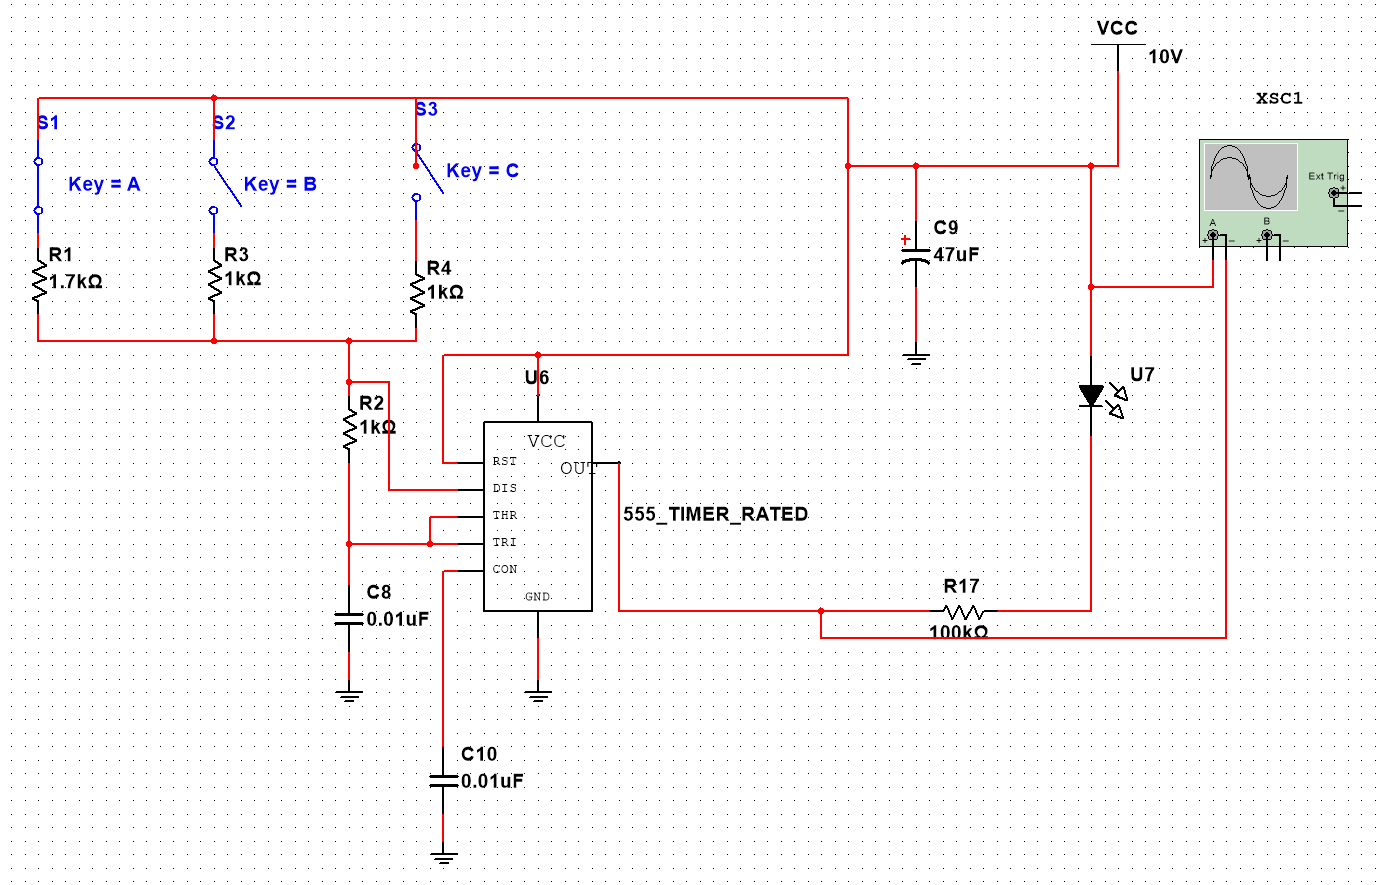
\includegraphics[width=1\textwidth]{4-1.png}
    \caption{红外发射Multisim仿真电路}
    \label{fig:xfig1}
\end{figure}

参数分析:

此处,我们使得RB为1k,为了产生使用NE555产生38kHz的方波信号。

由下式可知:

频率 = 0.693((RA+2RB)*C) 
占空比 = RB/(RA+2RB)

将RB=1k,C=0.01u带入得到

RA=1.7,因此我们需要1.7k的电阻。

此时输出的期望信号为38kHz、26.4\%占空比的方波。

~\\

其中U7为发光二极管,其参数如下:
\begin{figure}[H] % use float package if you want it here
    \centering
    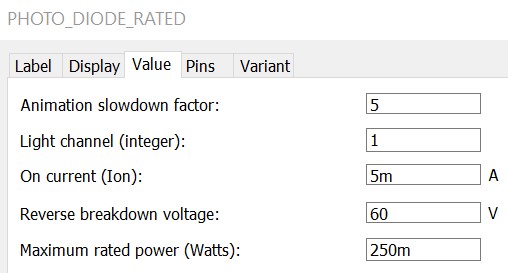
\includegraphics[width=0.5\textwidth]{4-2.png}
    \caption{U7参数}
    \label{fig:xfig1}
 \end{figure}
 ~\\

测量其输出电压波形如下:
\begin{figure}[H] % use float package if you want it here
    \centering
    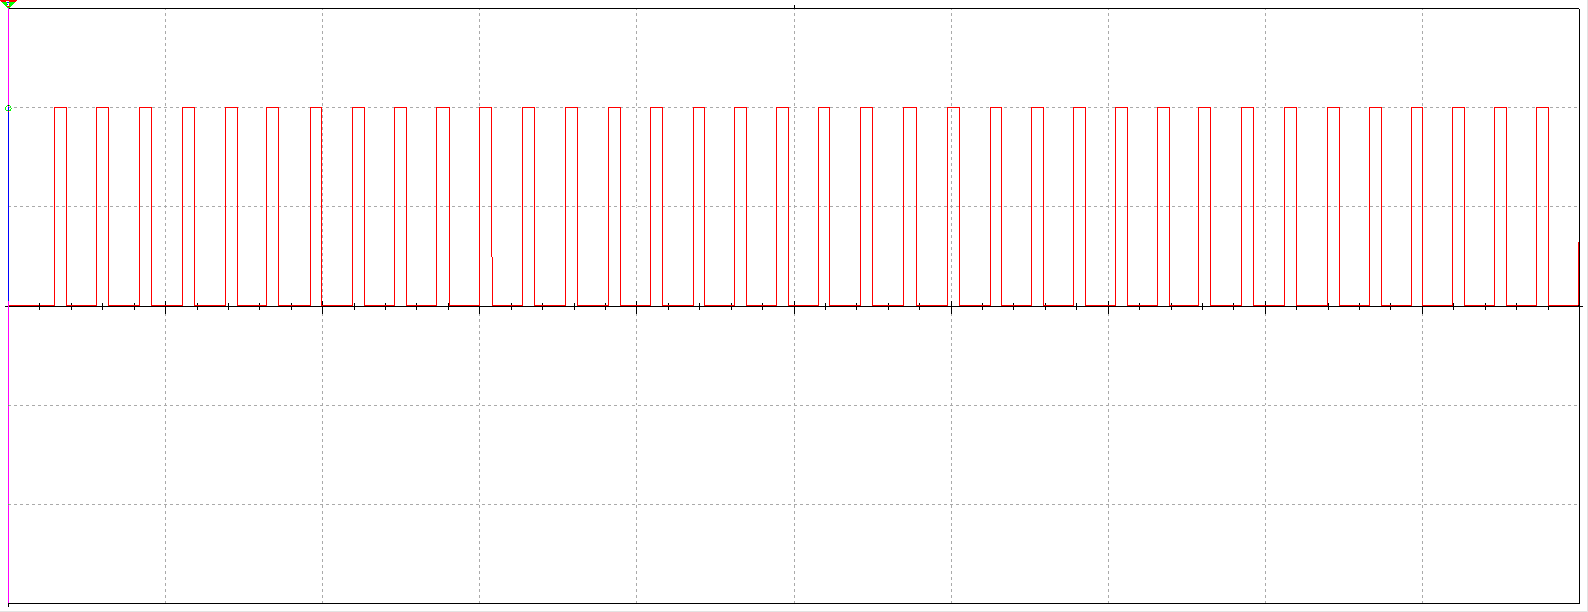
\includegraphics[width=0.8\textwidth]{4-3.png}
    \caption{红外发射整体波形}
    \label{fig:xfig1}
\end{figure}
\begin{figure}[H] % use float package if you want it here
    \centering
    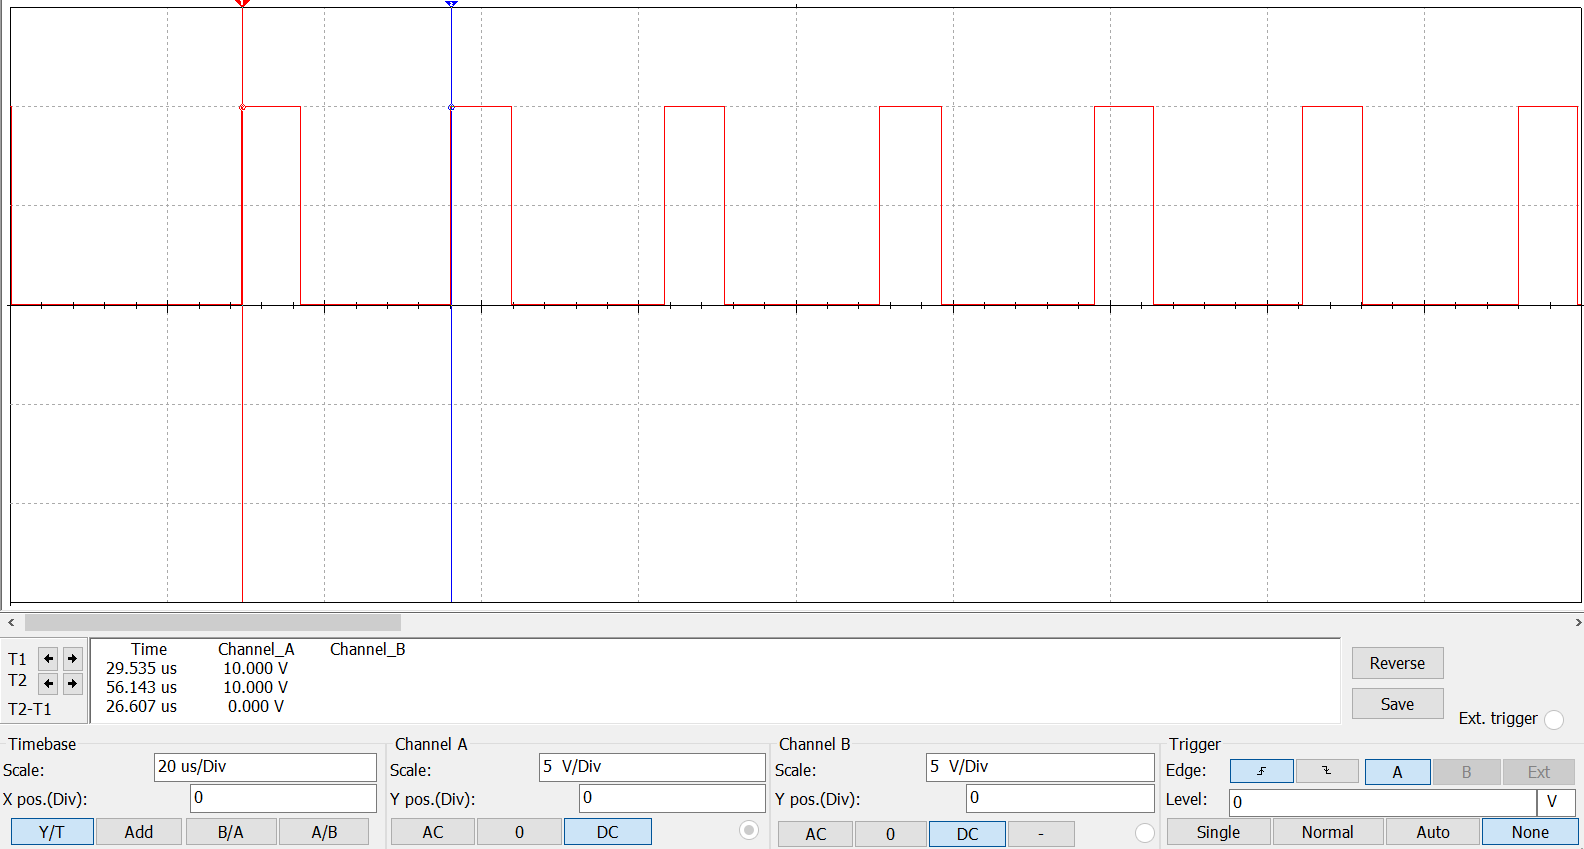
\includegraphics[width=0.8\textwidth]{4-4.png}
    \caption{红外发射周期}
    \label{fig:xfig1}
\end{figure}
\begin{figure}[H] % use float package if you want it here
    \centering
    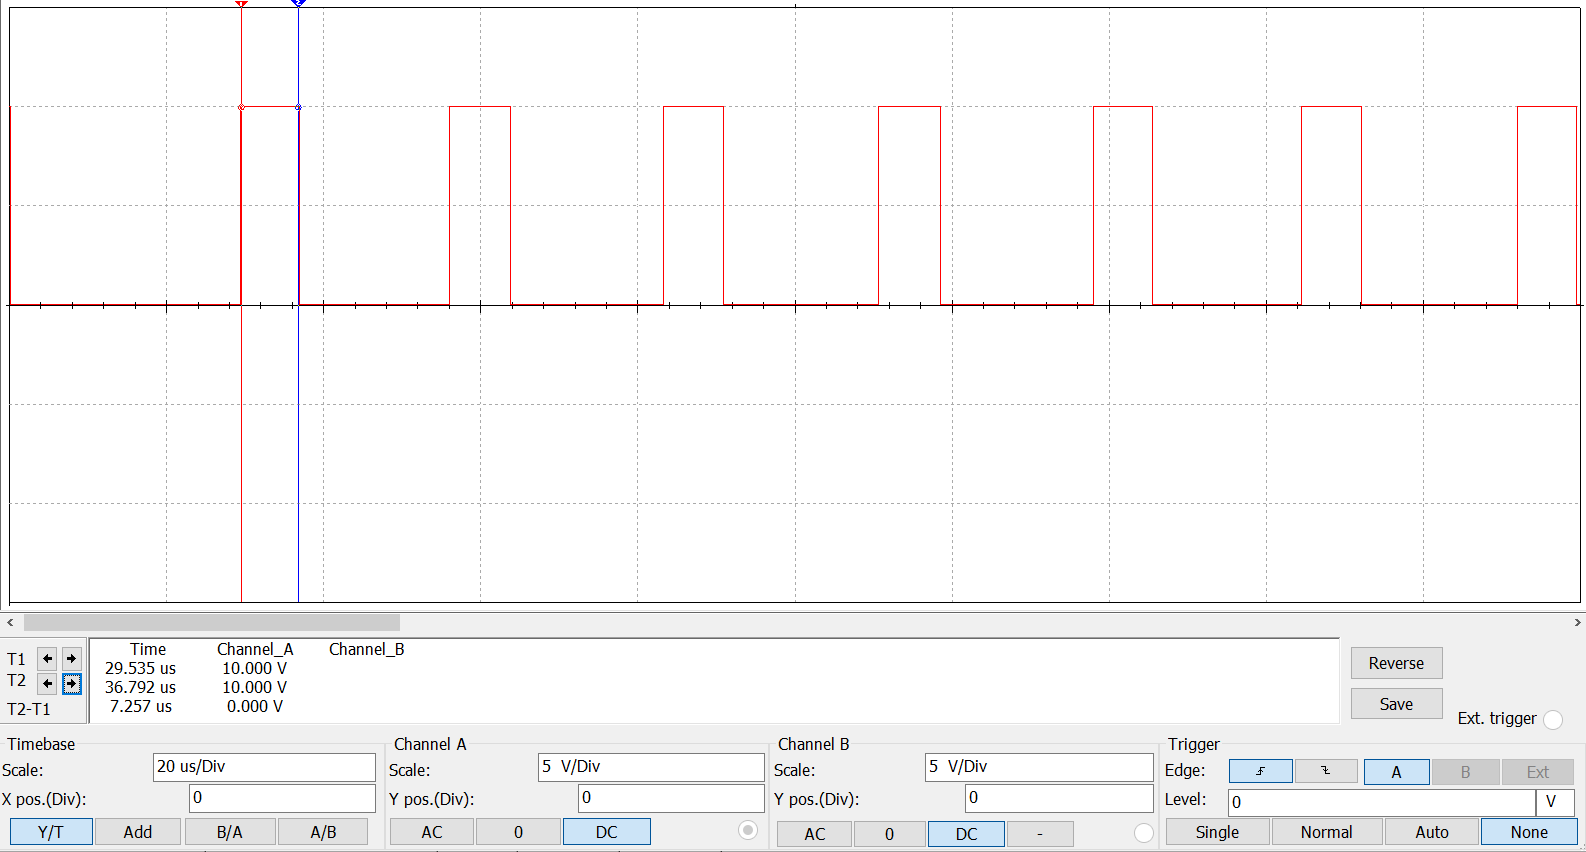
\includegraphics[width=0.8\textwidth]{4-5.png}
    \caption{红外发射占空比}
    \label{fig:xfig1}
\end{figure}



\section{红外接收Multisim仿真电路}
\begin{figure}[H] % use float package if you want it here
    \centering
    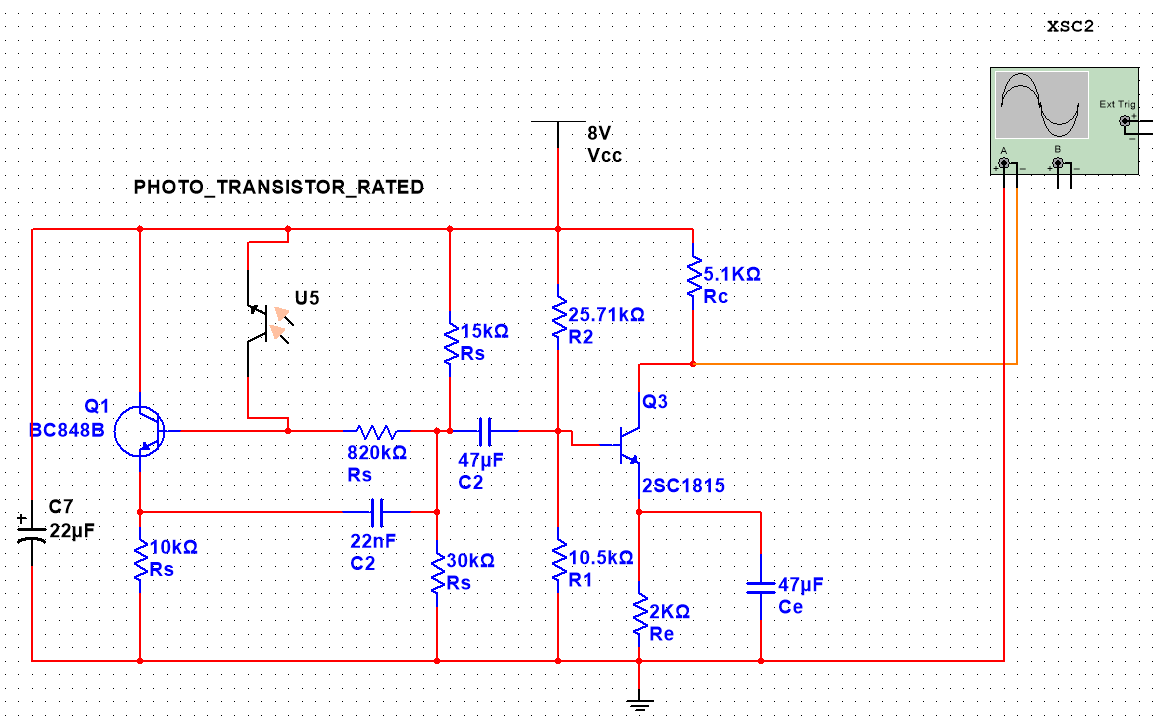
\includegraphics[width=1\textwidth]{5-1.png}
    \caption{红外接收Multisim仿真电路}
    \label{fig:xfig1}
\end{figure}

其中U5为发光二极管,其参数如下:

\begin{figure}[H] % use float package if you want it here
    \centering
    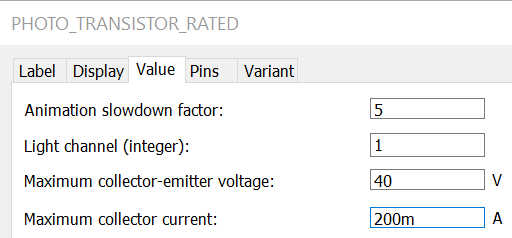
\includegraphics[width=0.5\textwidth]{5-2.png}
    \caption{U5参数}
    \label{fig:xfig1}
 \end{figure}

 ~\\

测量其输出电压波形如下:
\begin{figure}[H] % use float package if you want it here
    \centering
    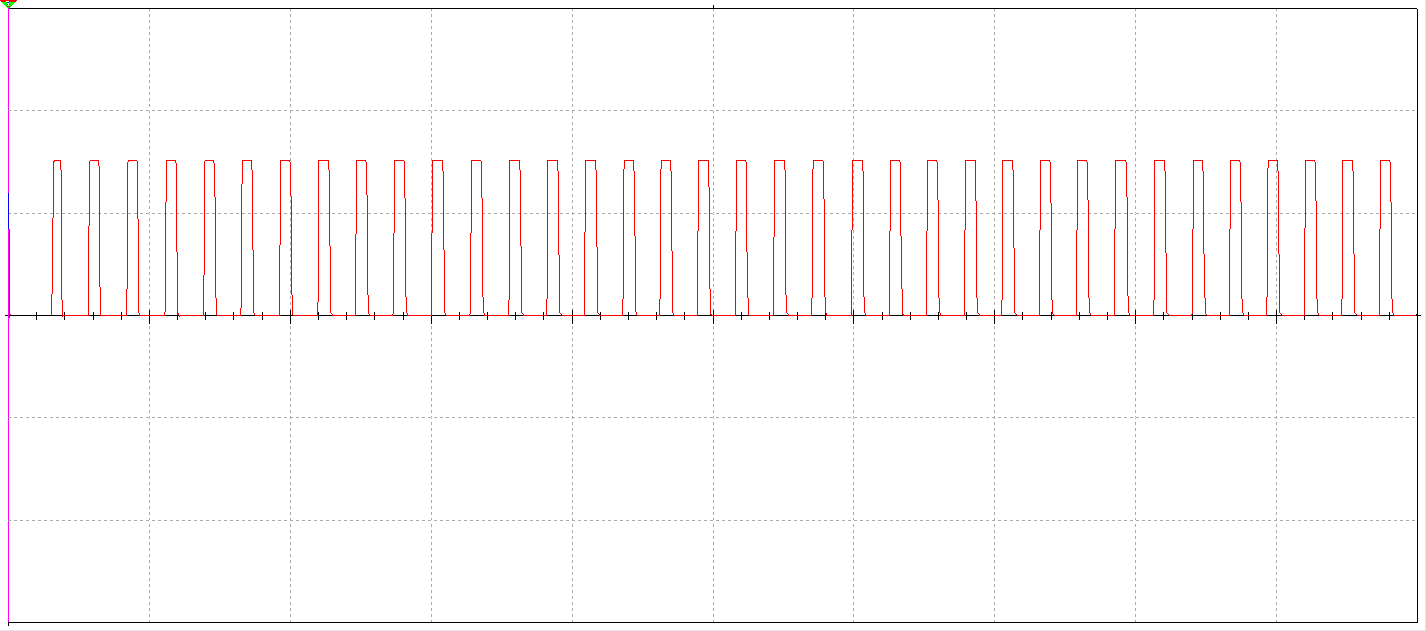
\includegraphics[width=0.8\textwidth]{5-3.png}
    \caption{红外接收整体波形}
    \label{fig:xfig1}
\end{figure}
\begin{figure}[H] % use float package if you want it here
    \centering
    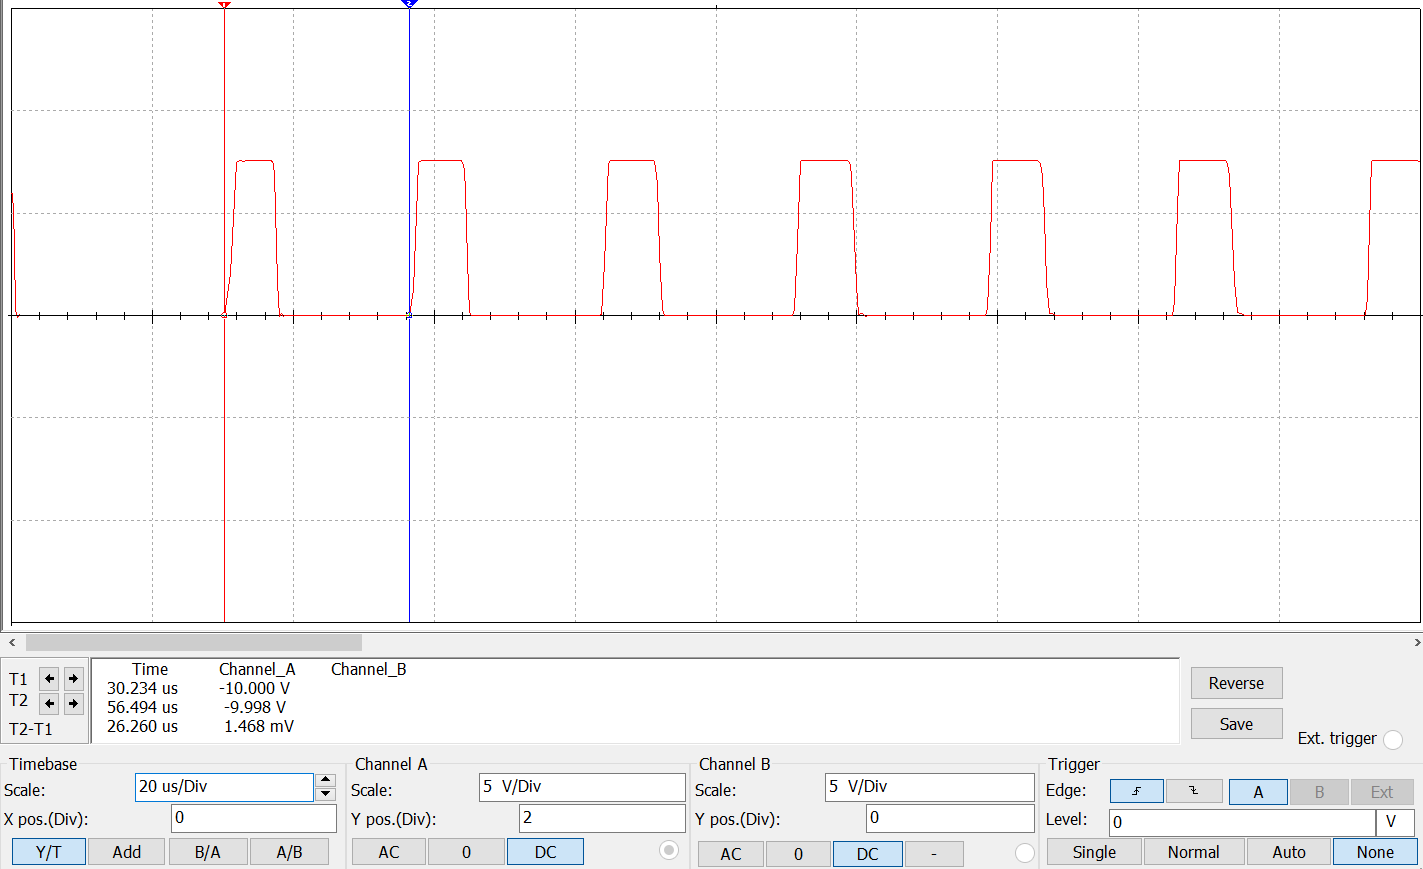
\includegraphics[width=0.8\textwidth]{5-4.png}
    \caption{红外接收周期}
    \label{fig:xfig1}
\end{figure}
\begin{figure}[H] % use float package if you want it here
    \centering
    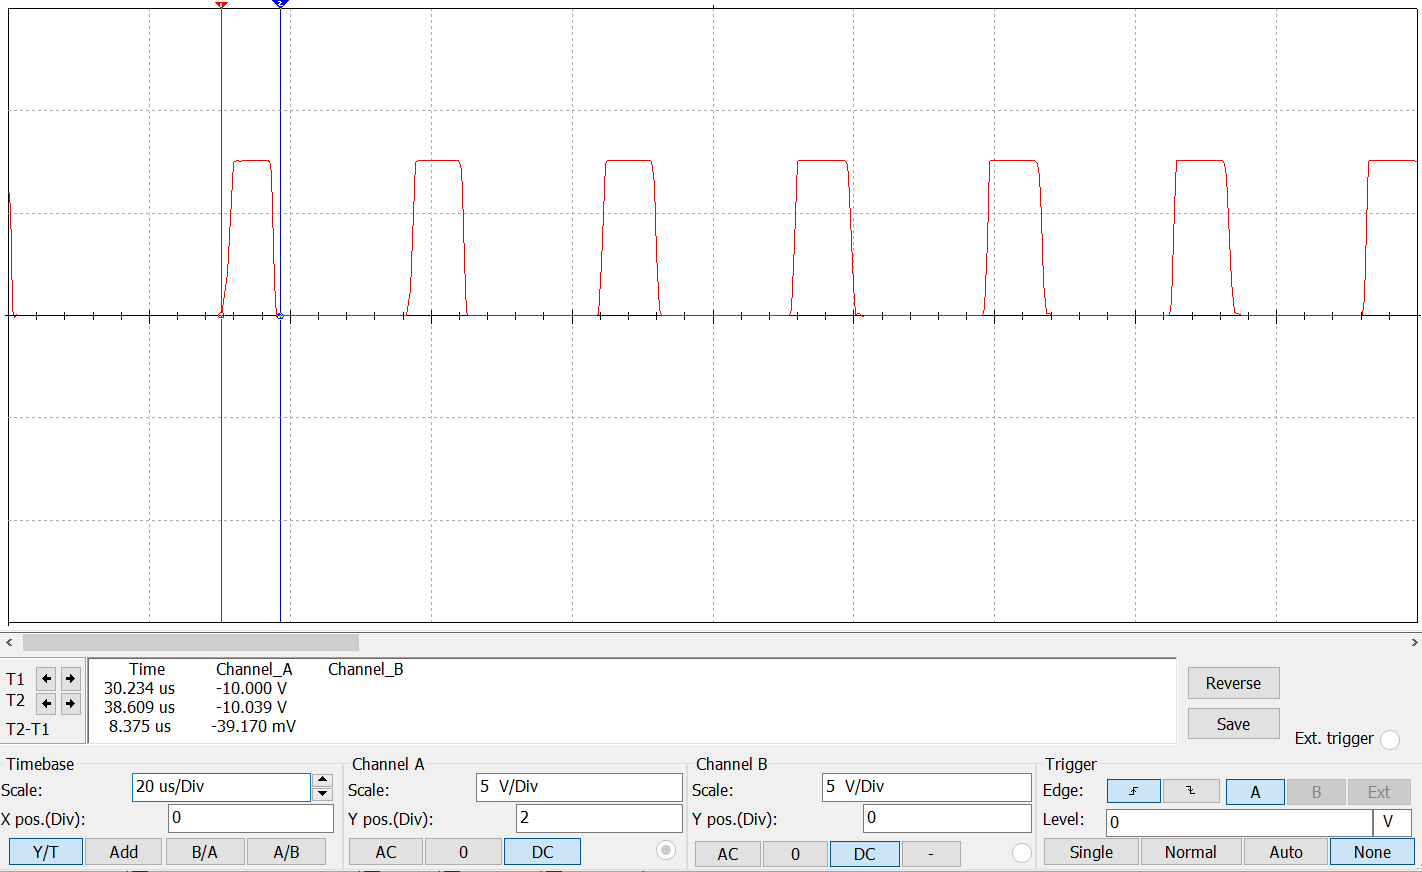
\includegraphics[width=0.8\textwidth]{5-5.png}
    \caption{红外接收占空比}
    \label{fig:xfig1}
\end{figure}

结果分析:\\
期望信号为38kHz、26.4\%占空比的方波。

实际红外发射信号周期为:26.607us,即频率为37.584kHz,误差为1.10\%

实际红外发射信号占空比为:7.257us/26.607us,即为27.27\%,误差为3.30\%

实际红外发射信号电压大小:10V

~\\

当以实际红外发射信号发射时,分析实际红外接收信号。

实际红外接收信号周期为:26.260us,即频率为38.08kHz,误差为1.30\%

实际红外接收信号占空比为:8.375us/26.260us,即为31.89\%,误差为16.94\%

实际红外接收信号电压大小:-20V,放大了-2倍

并且此时接收信号反映稍微的延时。因此实际占空比误差应该更小



均在误差允许范围之内,据此进行PCB的制作和设计结果分析。
